\section{Эксперимент BM@N}

\subsection{Моделирование отклика установки}

Разработанная физическая программа измерения коллективных потоков в эксперименте BM@N была проверена на реалистичном Монте-Карло моделировании отклика детектора. 
В качестве входных данных моделирования были использованы две физические модели столкновения тяжелых ионов.
Модель DCM-QGSM-SMM (Dubna Cascade Model, Quark-Gluon String Model, Statistical Multifragmentation Model)~\cite{Botvina:1994vj,Baznat:2019iom} реалистично описывает выход спектаторных фрагментов, однако неудовлетворительно воспроизводит коллективную анизотропию рожденных частиц.
Эта модель была использована для проверки разработанных методов вычисления поправочного коэффициента разрешения в эксперименте BM@N.

Модель JAM (Jet-A-A Model)~\cite{Nara:2016hbg,Nara:2019qfd,Nara:2020ztb} с импульсно-зависимым потенциалом MD3 дает реалистичный сигнал коллективной анизотропии рожденных барионов, однако в модели отсутствуют фрагменты с массовым номером $A>1$.
Данная модель была использована для проверки коррекций на неоднородность детектора и возможности алгоритмов реконструкции восстановить сигнал коллективной анизотропии.

В плоскости поперечной направлению пучка аксептанс установки имеет прямоугольную форму, что ведёт к значительной неоднородности аксептанса.
На рис.~\ref{fig:bmn_phi_eta} представлен азимутальный аксептанс заряженных частиц в зависимости от псевдобыстроты. 
%
\begin{figure}[ht]
\begin{center}
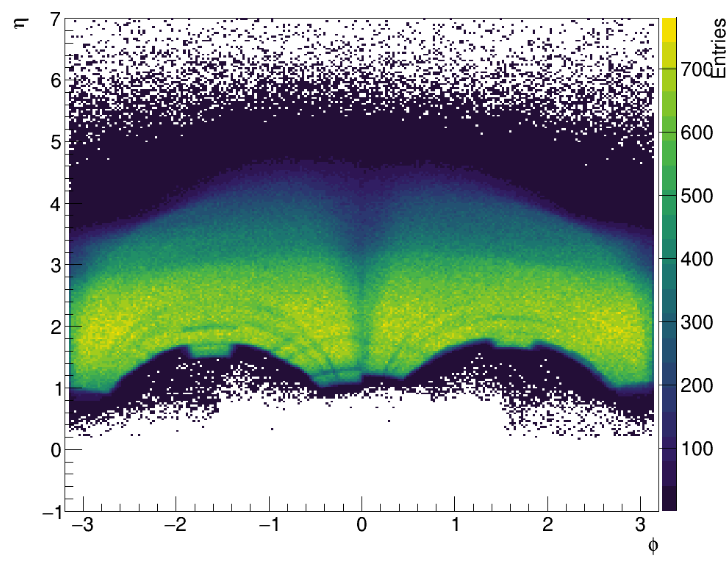
\includegraphics[width=0.55\linewidth]{images/bmn_phi_eta.png}
\caption{Азимутальный аксептанс заряженных частиц в зависимости от псевдобыстроты.}
\label{fig:bmn_phi_eta}
\end{center}
\end{figure}

На рис.~\ref{fig:bmn_mom_res} показано импульсное разрешение трекинговой системы как функция импульса частицы.
Различными цветами и маркерами показаны различные энергии столкновения ядер Xe и Cs.
Разрешение падает с уменьшением энергии столкновения. 
Этот эффект связан с уменьшением магнитного поля, при уменьшении энергии столкновения. 
При энергии $E_{kin}$=2$A$~ГэВ, экспериментальная установка работает с магнитным полем 0.4~Тл, при энергии $E_{kin}$=3$A$~ГэВ магнитное поле 0.6~Тл и при энергии $E_{kin}$=4$A$~ГэВ --- 0.8~Тл.
%
\begin{figure}[ht]
\begin{center}
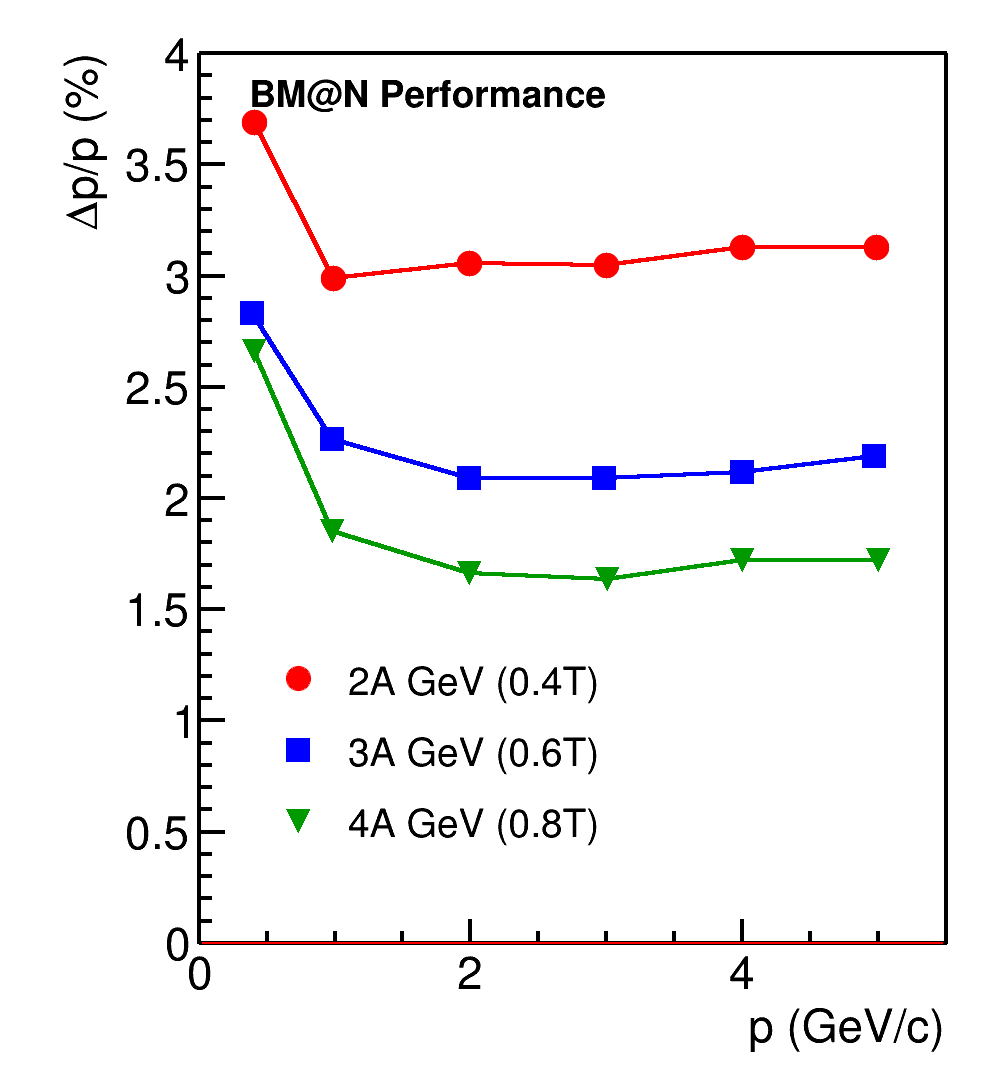
\includegraphics[width=0.55\linewidth]{images/momentum_resolution.png}
\caption{Разрешение трекинговой системы по импульсу в эксперименте BM@N. Различными цветами и маркерами показана различная энергия столкновения.}
\label{fig:bmn_mom_res}
\end{center}
\end{figure}

\subsection{Определение центральности}

В эксперименте BM@N центральность была определена при помощи метода Монте-Карло Глаубера, в качестве множественности использовалось число восстановленных траекторий заряженных частиц~\cite{Segal:2023njv}.
В качестве параметров распределения Вудса-Саксона (\ref{eq:woods_saxon}) использовались следющие значения: Xe ($A=129$, $Z=54$, $R=5.46$~фм, $a=0.57$~фм) и Cs ($A=133$, $Z=55$, $R=6.125$~фм, $a=0.5$~фм).
Далее согласно процедуре, описанной в секции~\ref{theory:centrality}, были разыграны параметры $N_{part}$, $N_{col}$ и путем варьирования $f$, $\mu$ и $k$ достигалось наилучшее согласие смоделированной множественности с экспериментальной.
Восстановленное методом МК-Глаубера распределение множественности при полном сечении неупругого взаимодействия было разбито на классы центральности по 5\% и 10\%.

На рис.~\ref{fig:bmn_multiplicity} слева представлено распределение множественности заряженных частиц для Монте-Карло моделирования столкновений Xe+Cs(I) при энергии $E_{kin}$=4$A$~ГэВ.
Открытыми маркерами обозначено распределение множественности заряженных траекторий после полной цепочки реконструкции событий модели DCM-QGSMSMM.
Синими треугольниками представлено распределение множественности полученное методом МК-Глаубра.
Вертикальными линиями обозначены границы классов центральности.
Модель Монте-Карло Глаубера хорошо описывает распределение множественности в границах 0-80\% класса центральности.
Справа представлены значения среднего прицельного параметра в каждом классе центральности по множественности.
Открытые символы обозначают значения, полученные из модели DCM-QGSMSMM.
Синие треугольники --- значение, извлеченные из модели МК-Глаубера.
Наблюдается хорошее согласие между реконструированными значениями прицельного параметра и настоящими из DCM-QGSMSMM.
%
\begin{figure}[ht]
\begin{center}
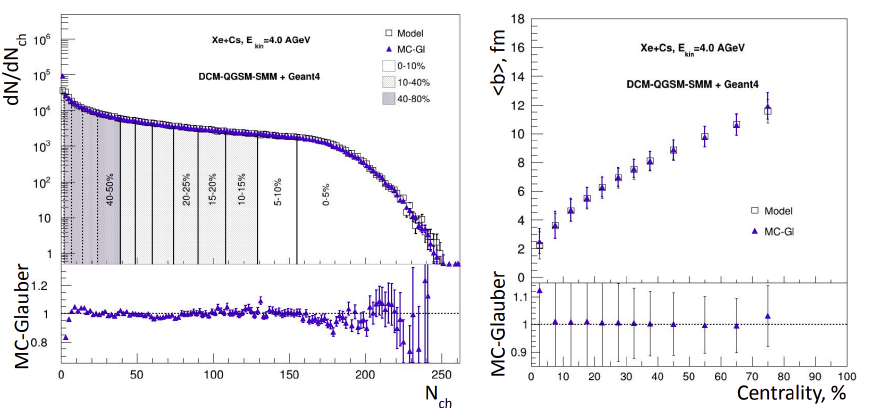
\includegraphics[width=0.95\linewidth]{images/mc_glauber_xecs_mult.png}
\caption{Слева: распределение множественности заряженных частиц в эксперименте BM@N. Вертикальными линиями изображены границы классов центральности. Справа: значения среднего прицельного параметра в классах центральности, определенных по множественности.}
\label{fig:bmn_multiplicity}
\end{center}
\end{figure}

\subsection{Идентификация протонов}

Для каждого из детекторов была построена зависимость квадрата массы делённого на квадрат заряда $m^2/q^2$ от импульса $p/q$. 
На рис.~\ref{fig:bmn_m2_pq} сверху, представлено распределение квадрата массы заряженной частицы в зависимости от импульса $p/q$ для TOF-400 (слева) и TOF-700 (справа).
В узких диапазонах поперечного импульса распределение частиц по квадрату массы было аппроксимировано гауссовой функцией. 
На рис.~\ref{fig:bmn_m2_pq} снизу, представлены кандидаты в протоны, которые лежат не дальше $2\sigma$ от пика квадрата массы.
%
\begin{figure}[ht]
\begin{center}
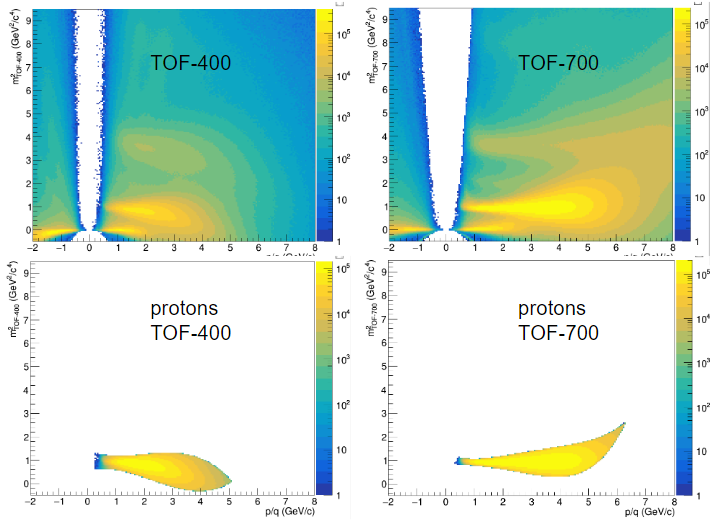
\includegraphics[width=0.95\linewidth]{images/bmn_m2_pq.png}
\caption{Распределение квадрата массы деленного на квадрат заряда заряженной частицы в зависимости от импульса $p/q$ для TOF-400 (слева) и TOF-700 (справа). Сверху представлены распределения для всех заряженных частиц, снизу --- для отобранных протонов.}
\label{fig:bmn_m2_pq}
\end{center}
\end{figure}


На рис.~\ref{fig:bmn_pt_y} представлено распределение протонов по быстроте $y_{cm}$ и поперечному импульсу $p_T$ идентифицированных при помощи TOF-400 (слева сверху), TOF-700 (слева снизу), с использованием обоих TOF-детекторов (справа).
%
\begin{figure}[ht]
\begin{center}
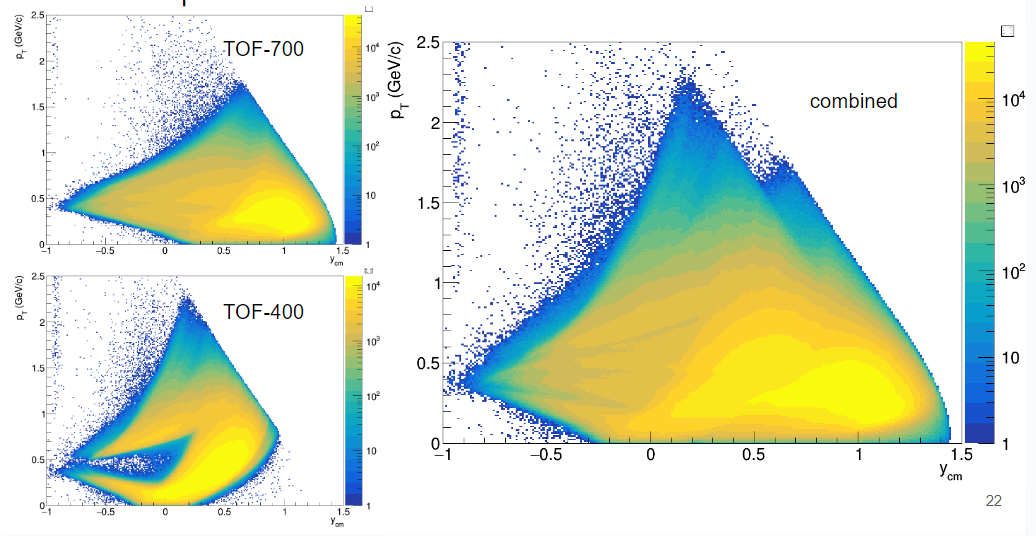
\includegraphics[width=0.95\linewidth]{images/bmn_pt_y_acceptance.png}
\caption{Распределение протонов по быстроте $y_{cm}$ и поперечному импульсу $p_T$, идентифицированных при помощи TOF-400 (слева сверху), TOF-700 (слева снизу), с использованием обоих TOF-детекторов (справа).}
\label{fig:bmn_pt_y}
\end{center}
\end{figure}


\subsection{Кинематические окна, в которых были определены $Q_1$-вектора}

Для восстановления плоскости симметрии в эксперименте BM@N была использована информация с калориметра FHCal.
Модули детектора были разделены на 3 группы согласно их псевдобыстроте (F1, F2 и F3).
Схематические группы модулей изображены различными цветами на рис.~\ref{fig:bmn_subevents} слева.

Дополнительно для исследования вклада непотоковых корреляций в измеренные значения коллективной анизотропии были введены два $Q_1$-вектора из треков заряженных частиц. 
Вектор $Tp$ построен для протонов со значениями быстроты $0.4<y_{cm}<0.6$ и поперечным импульсом $0.2<p_{T}<2.0$~$GeV/c$.
Вектор $T\pi$ формировался для отрицательных пионов с быстротой и поперечным импульсом $0.2<y_{cm}<0.8$ и $0.1<p_T<0.5 GeV/c$ соответственно.
Соответствующие кинематические области изображены красными прямоугольниками на рис.~\ref{fig:bmn_subevents} справа.
%
\begin{figure}[ht]
\begin{center}
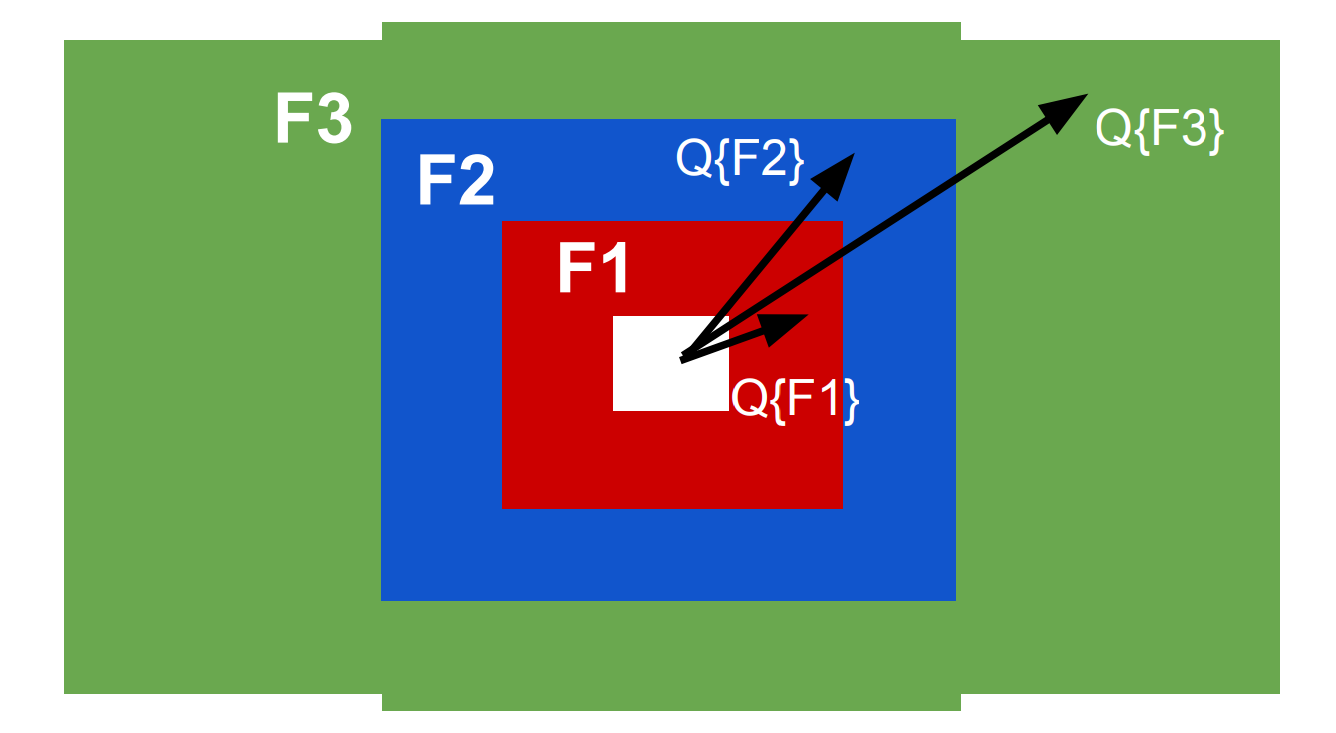
\includegraphics[width=0.45\linewidth]{images/FHCal_layout.png}
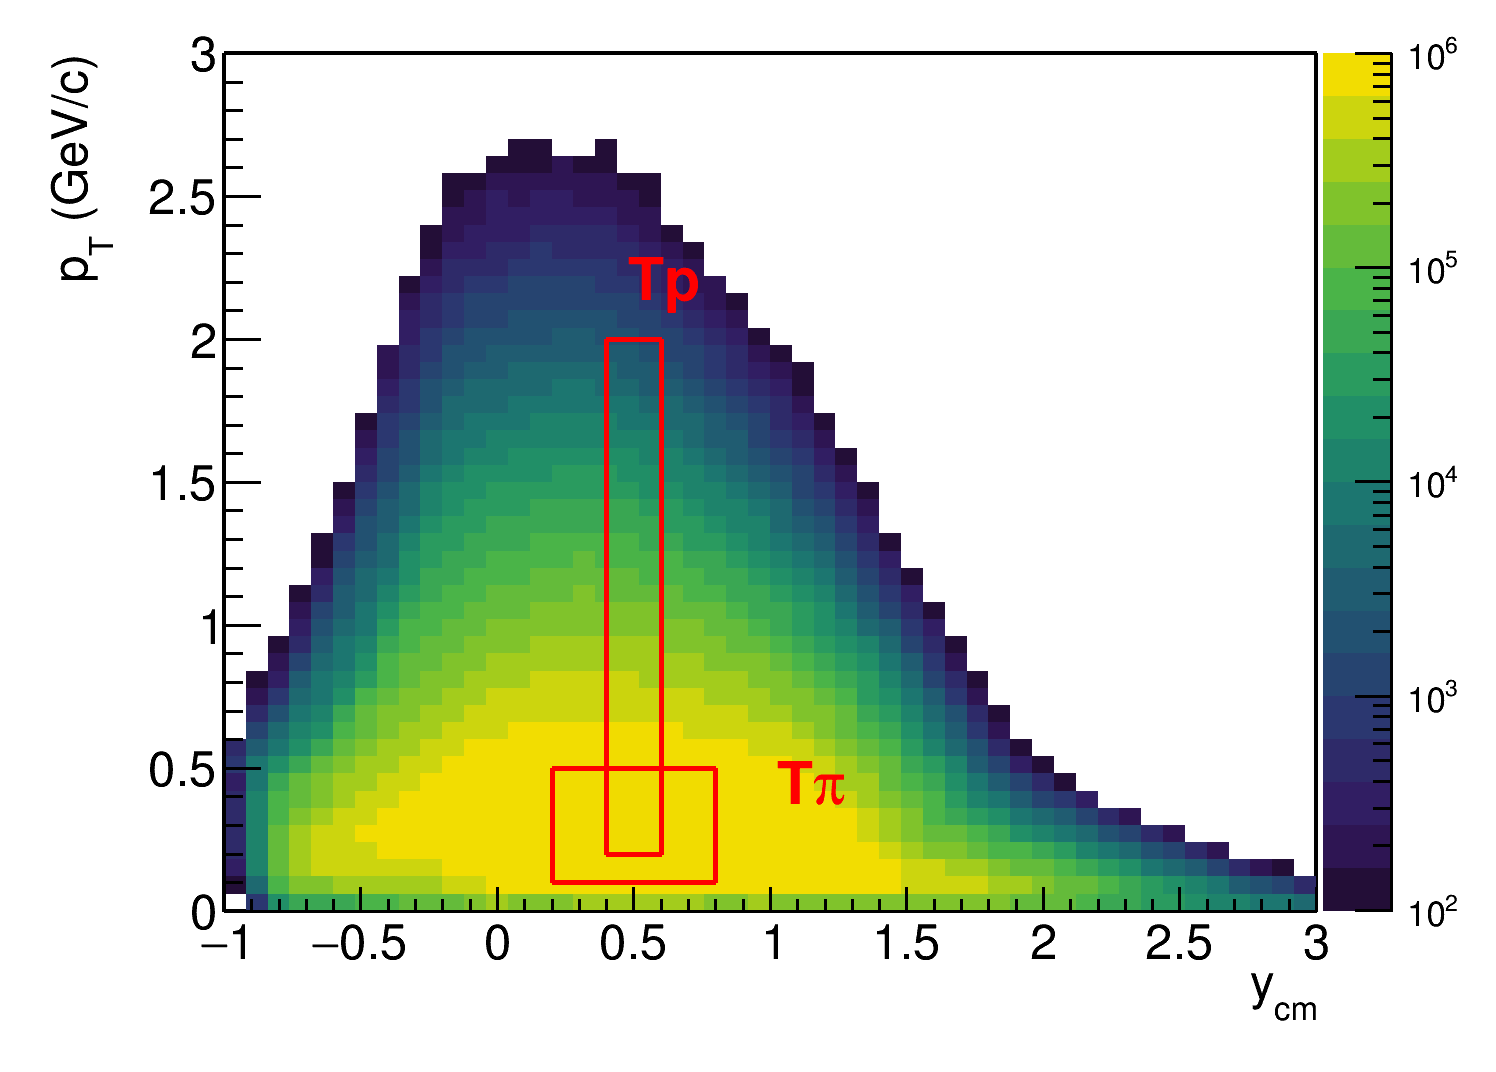
\includegraphics[width=0.45\linewidth]{images/pT_ycm_protons.png}
\caption{
Слева: Схема разделения модулей переднего адронного калориметра по группам для определения плоскости симметрии события.
Справа: Кинематические окна для подсчета $Q_1$-векторов из треков заряженных частиц.
}
\label{fig:bmn_subevents}
\end{center}
\end{figure}

\subsection{Коррекция на азимутальную неоднородность аксептанса установки}

Эффект применения коррекций на азимутальную неоднородность детектора представлен на рис~\ref{fig:bmn_components}~\cite{Mamaev:2023yhz}.
%
\begin{figure}[ht]
\begin{center}
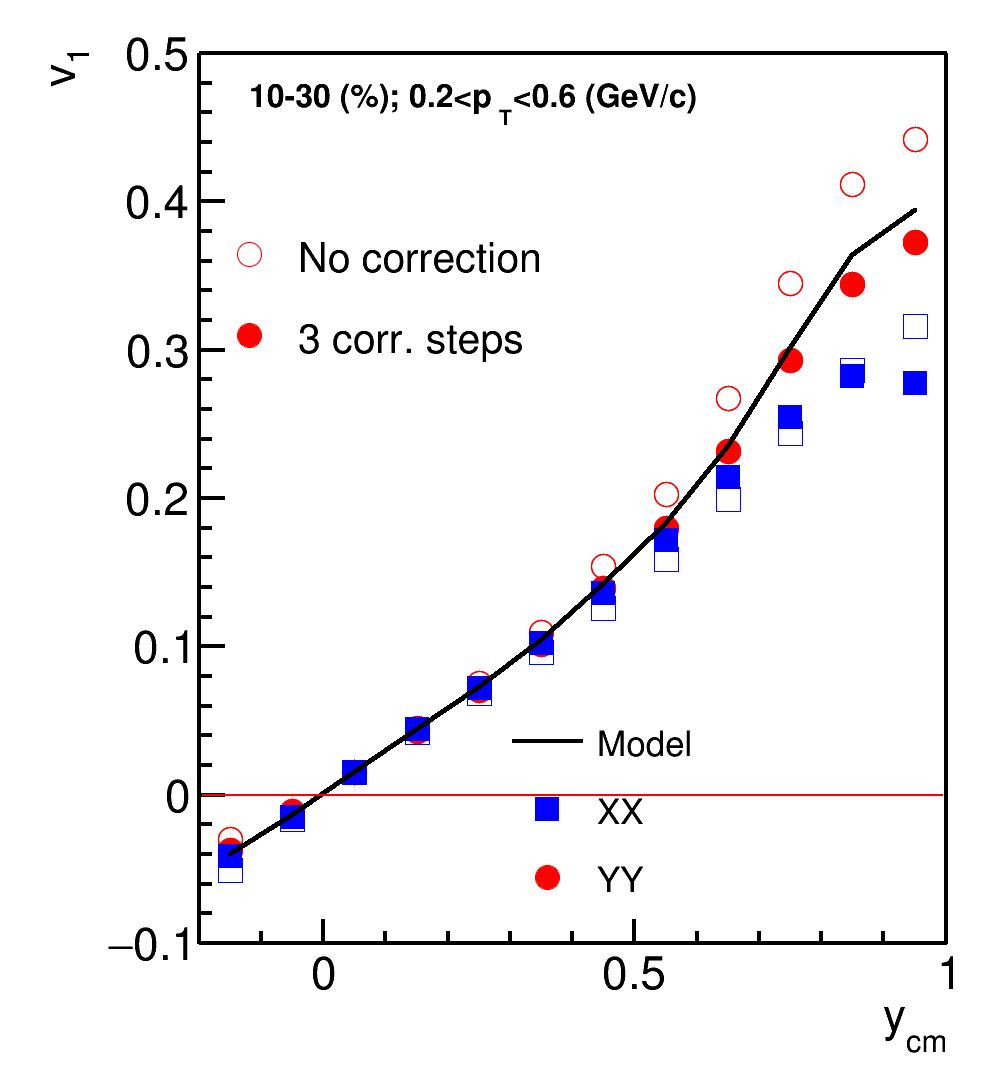
\includegraphics[width=0.45\linewidth]{images/v1_proton_correction_rapidity.png}
\caption{Сравнение направленного потока $v_1$ протонов рожденных в Монте-Карло моделировании столкновений Xe+Cs в эксперименте BM@N. Направленный поток получен с использованием различных компонент $u_1$-вектора. Разными маркерами обозначены результаты до и после коррекции на азимутальную неоднородность аксептанса детектора. }
\label{fig:bmn_components}
\end{center}
\end{figure}

Результаты получены для реалистичного моделирования отклика детектора с использованием программного пакета GEANT4.
Разными цветами обозначен результат $v_1$ протонов, полученный с использованием различных компонент $u_1$-вектора. 
Маркеры обозначают результаты до и после коррекции на азимутальную неоднородность детектора.
Черной линией обозначена зависимость $v_1$ протонов извлеченная напрямую из модели без реконструкции.
После применения 3 ступеней коррекции, результаты полученные при помощи $YY$ корреляции $u_1$ и $Q_1$-векторов, хорошо согласуются с результатами извлеченными напрямую из модели.
Напротив, $v_1$, посчитанный с использованием $XX$-компонент, расходится с модельной зависимостью $v_1$ от быстроты. 
Причиной может служить отклонение частиц в направлении оси $x$ в магнитном поле. 
В связи с этим, в дальнейшем для анализа будет использованы лишь корреляции $YY$-компонент $u_1$ и $Q_1$-векторов.


\section{Выводы к главе 3}

В главе описаны методы определения центральности и идентификации протонов с помощью экспериментальной установки HADES.
Представлены критерии отбора столкновений Au+Au и Ag+Ag а также заряженных частиц, рожденных в этих столкновениях.
Описаны способы вычисления эффективности реконструкции протонов при помощи программного пакета GEANT3.
В главе обсуждаются методы определения плоскости симметрии столкновения а также способы вычисления разрешения плоскости симметрии при помощи переднего годоскопа FW в эксперименте HADES.
Приводятся результаты применения коррекций на азимутальную анизотропию аксептанса установки HADES и обсуждаются остаточные систематические погрешности, связанные с этим эффектом.
В главе приводится детальное описание процесса вычисления систематической ошибки, связанной с непотоковыми корреляциями, включенными в финальный опубликованный результат~\cite{HADES:2020lob}.
Произведено сравнение методов вычисления $v_1$: методов плоскости события и скалярного произведения и систематическая разница оказалась в пределах статистической ошибки.
Сравнение направленного потока протонов, измеренных при помощи метода случайных и метода трех подсобытий показывает систматическую разницу порядка 5\% для среднецентральных столкновений ядер Au+Au.
Использование метода случайных подсобытий для вычисления $v_1$ протонов в столкновениях ядер Ag+Ag даёт большую систематическую ошибку, которая может достигать 15\%.
На основании этих оценок, была вычислена систематическая ошибка на измеренные значения коллективных потоков протонов, включенная в публикацию~\cite{HADES:2020lob}.

Для экспериментальной установки BM@N описываются методы измерения центральности столкновения по числу треков заряженных частиц. 
В главе обсуждаются способы измерения производительности установки BM@N для измерения направленного и эллиптического потоков протонов с помощью физических Монте-Карло моделей столкновений тяжелых ионов и программного пакета GEANT4.
В главе представлены значения поправочного коэффициента разрешения $R_1$ для плоскостей симметрии, определенных при помощи переднего годоскопа FW.
Обсуждаются методы минимизации систематической ошибки связанной с непотоковыми корреляциями и вычисляется остаточная систематическая ошибка.
В главе представлены кинематические диапазоны, использованные для вычисления $Q_1$-векторов в Монте-Карло симуляции эксперимента BM@N.